
Se desea trabajar con series temporales sobre mediciones climatológicas. 
En concreto, se eligen las variables de temperatura del aire, humedad ambiental y presión atmosférica en la superficie.
Dichas variables son estudiadas con periodicidad horaria, en el intervalo comprendido entre el 1 de marzo de 2023 y el 28 de febrero de 2025.
\section{Fuentes de los datos}

Se han empleado 2 fuentes para recopilar las mediciones: 
\begin{itemize}
    \item \textbf{Grafcan}: Cartográfica de Canarias, S.A. es una empresa pública de la Comunidad Autónoma de Canarias.
    \item \textbf{Open-Meteo}: API pública de código abierto que proporciona datos de múltiples servicios de meteorología.
\end{itemize}

Se eligen 3 ubicaciones de la isla de Tenerife con distintas características climáticas:
\begin{itemize}
    \item \textbf{San Cristóbal de La Laguna}: La Cuesta, 35 metros de altitud.
    \item \textbf{La Orotava}: Camino de Chasna, 812 m.
    \item \textbf{Arona}: Punta de Rasca, 25m.
\end{itemize}
Dichas ubicaciones han sido elegidas al contar con estaciones de medición de Grafcan.
Sus posiciones se muestran en la Figura \ref{mapa_estaciones}.

Inicialmente se valoró emplear la estación correspondiente a Los Cristianos, en vez de la de Arona, pero se detectó que existía un período prolongado con datos faltantes, por lo que fue descartada.
\bigskip

\section{Proceso de adquisición}

Se estudian distintas alternativas para el almacenamiento de los datos.
Se opta por emplear TimescaleDB, una extensión del popular sistema PostgreSQL
de bases de datos relacionales, especialmente adaptada para el manejo de series temporales. 

\begin{figure}[htb]
   \centering
   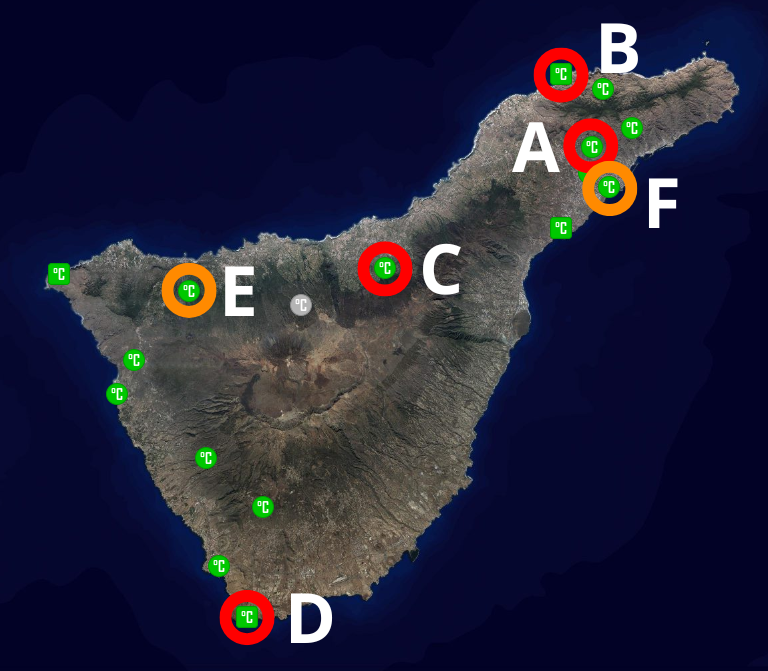
\includegraphics[width=0.6\linewidth]{images/mapa_estaciones}
   \caption{Mapa de las estaciones climatológicas Grafcan empleadas, señaladas en rojo. De izquierda a derecha: Arona, La Orotava y San Cristóbal de La Laguna.}
   \label{mapa_estaciones}
\end{figure}